% Template for PLoS
% Version 3.5 March 2018
%
% % % % % % % % % % % % % % % % % % % % % %
%
% -- IMPORTANT NOTE
%
% This template contains comments intended 
% to minimize problems and delays during our production 
% process. Please follow the template instructions
% whenever possible.
%
% % % % % % % % % % % % % % % % % % % % % % % 
%
% Once your paper is accepted for publication, 
% PLEASE REMOVE ALL TRACKED CHANGES in this file 
% and leave only the final text of your manuscript. 
% PLOS recommends the use of latexdiff to track changes during review, as this will help to maintain a clean tex file.
% Visit https://www.ctan.org/pkg/latexdiff?lang=en for info or contact us at latex@plos.org.
%
%
% There are no restrictions on package use within the LaTeX files except that 
% no packages listed in the template may be deleted.
%
% Please do not include colors or graphics in the text.
%
% The manuscript LaTeX source should be contained within a single file (do not use \input, \externaldocument, or similar commands).
%
% % % % % % % % % % % % % % % % % % % % % % %
%
% -- FIGURES AND TABLES
%
% Please include tables/figure captions directly after the paragraph where they are first cited in the text.
%
% DO NOT INCLUDE GRAPHICS IN YOUR MANUSCRIPT
% - Figures should be uploaded separately from your manuscript file. 
% - Figures generated using LaTeX should be extracted and removed from the PDF before submission. 
% - Figures containing multiple panels/subfigures must be combined into one image file before submission.
% For figure citations, please use "Fig" instead of "Figure".
% See http://journals.plos.org/plosone/s/figures for PLOS figure guidelines.
%
% Tables should be cell-based and may not contain:
% - spacing/line breaks within cells to alter layout or alignment
% - do not nest tabular environments (no tabular environments within tabular environments)
% - no graphics or colored text (cell background color/shading OK)
% See http://journals.plos.org/plosone/s/tables for table guidelines.
%
% For tables that exceed the width of the text column, use the adjustwidth environment as illustrated in the example table in text below.
%
% % % % % % % % % % % % % % % % % % % % % % % %
%
% -- EQUATIONS, MATH SYMBOLS, SUBSCRIPTS, AND SUPERSCRIPTS
%
% IMPORTANT
% Below are a few tips to help format your equations and other special characters according to our specifications. For more tips to help reduce the possibility of formatting errors during conversion, please see our LaTeX guidelines at http://journals.plos.org/plosone/s/latex
%
% For inline equations, please be sure to include all portions of an equation in the math environment.  For example, x$^2$ is incorrect; this should be formatted as $x^2$ (or $\mathrm{x}^2$ if the romanized font is desired).
%
% Do not include text that is not math in the math environment. For example, CO2 should be written as CO\textsubscript{2} instead of CO$_2$.
%
% Please add line breaks to long display equations when possible in order to fit size of the column. 
%
% For inline equations, please do not include punctuation (commas, etc) within the math environment unless this is part of the equation.
%
% When adding superscript or subscripts outside of brackets/braces, please group using {}.  For example, change "[U(D,E,\gamma)]^2" to "{[U(D,E,\gamma)]}^2". 
%
% Do not use \cal for caligraphic font.  Instead, use \mathcal{}
%
% % % % % % % % % % % % % % % % % % % % % % % % 
%
% Please contact latex@plos.org with any questions.
%
% % % % % % % % % % % % % % % % % % % % % % % %

\documentclass[10pt,letterpaper]{article}
\usepackage[top=0.85in,left=2.75in,footskip=0.75in]{geometry}

% amsmath and amssymb packages, useful for mathematical formulas and symbols
\usepackage{amsmath,amssymb}

% Use adjustwidth environment to exceed column width (see example table in text)
\usepackage{changepage}

% Use Unicode characters when possible
\usepackage[utf8x]{inputenc}

% textcomp package and marvosym package for additional characters
\usepackage{textcomp,marvosym}

% cite package, to clean up citations in the main text. Do not remove.
\usepackage{cite}

% Use nameref to cite supporting information files (see Supporting Information section for more info)
\usepackage{nameref,hyperref}

% line numbers
\usepackage[right]{lineno}

% ligatures disabled
\usepackage{microtype}
\DisableLigatures[f]{encoding = *, family = * }

% color can be used to apply background shading to table cells only
\usepackage[table]{xcolor}

% array package and thick rules for tables
\usepackage{array}

% create "+" rule type for thick vertical lines
\newcolumntype{+}{!{\vrule width 2pt}}

% create \thickcline for thick horizontal lines of variable length
\newlength\savedwidth
\newcommand\thickcline[1]{%
  \noalign{\global\savedwidth\arrayrulewidth\global\arrayrulewidth 2pt}%
  \cline{#1}%
  \noalign{\vskip\arrayrulewidth}%
  \noalign{\global\arrayrulewidth\savedwidth}%
}

% \thickhline command for thick horizontal lines that span the table
\newcommand\thickhline{\noalign{\global\savedwidth\arrayrulewidth\global\arrayrulewidth 2pt}%
\hline
\noalign{\global\arrayrulewidth\savedwidth}}


% Remove comment for double spacing
%\usepackage{setspace} 
%\doublespacing

% Text layout
\raggedright
\setlength{\parindent}{0.5cm}
\textwidth 5.25in 
\textheight 8.75in

% Bold the 'Figure #' in the caption and separate it from the title/caption with a period
% Captions will be left justified
\usepackage[aboveskip=1pt,labelfont=bf,labelsep=period,justification=raggedright,singlelinecheck=off]{caption}
\renewcommand{\figurename}{Fig}

%ALK packages
\usepackage{placeins}
\usepackage{rotating}
\usepackage{tabularx}
\usepackage{longtable}
% \usepackage{natbib}

% Use the PLoS provided BiBTeX style
\bibliographystyle{plos2015}

% Remove brackets from numbering in List of References
\makeatletter
\renewcommand{\@biblabel}[1]{\quad#1.}
\makeatother



% Header and Footer with logo
\usepackage{lastpage,fancyhdr,graphicx}
\usepackage{epstopdf}
%\pagestyle{myheadings}
\pagestyle{fancy}
\fancyhf{}
%\setlength{\headheight}{27.023pt}
%\lhead{\includegraphics[width=2.0in]{PLOS-submission.eps}}
\rfoot{\thepage/\pageref{LastPage}}
\renewcommand{\headrulewidth}{0pt}
\renewcommand{\footrule}{\hrule height 2pt \vspace{2mm}}
\fancyheadoffset[L]{2.25in}
\fancyfootoffset[L]{2.25in}
\lfoot{\today}

%% Include all macros below

\newcommand{\lorem}{{\bf LOREM}}
\newcommand{\ipsum}{{\bf IPSUM}}

%% END MACROS SECTION


\begin{document}
\vspace*{0.2in}

% Title must be 250 characters or less.
\begin{flushleft}
{\Large
\textbf\newline{Development of a quantitative PCR assay for the detection and enumeration of a potentially ciguatoxin-producing dinoflagellate, \emph{Gambierdiscus lapillus} (Gonyaulacales, Dinophyceae).} % Please use "sentence case" for title and headings (capitalize only the first word in a title (or heading), the first word in a subtitle (or subheading), and any proper nouns).
}
\newline
% Insert author names, affiliations and corresponding author email (do not include titles, positions, or degrees).
\\
Anna Liza Kretzschmar\textsuperscript{1,2},
Arjun Verma\textsuperscript{2},
Gurjeet Kohli\textsuperscript{2},
Shauna Murray\textsuperscript{2,3}
\\
\bigskip
\textbf{1} Affiliation ithree institute, University of Technology Sydney, Ultimo, NSW, Australia
\\
\textbf{2} Affiliation climate change cluster, University of Technology Sydney, Ultimo, NSW, Australia
\\
\textbf{3} Affiliation Alfred Wegener-Institut Helmholtz-Zentrum für Polar- und Meeresforschung, Am Handelshafen 12, 27570, Bremerhaven, Germany
%\\
\bigskip

% Insert additional author notes using the symbols described below. Insert symbol callouts after author names as necessary.
% 
% Remove or comment out the author notes below if they aren't used.
%
% Primary Equal Contribution Note
%\Yinyang These authors contributed equally to this work.

% Additional Equal Contribution Note
% Also use this double-dagger symbol for special authorship notes, such as senior authorship.
%\ddag These authors also contributed equally to this work.

% Current address notes
%\textcurrency Current Address: Dept/Program/Center, Institution Name, City, State, Country % change symbol to "\textcurrency a" if more than one current address note
% \textcurrency Previous Address: 
% \textcurrency c Insert third current address

% Deceased author note
%\dag Deceased

% Group/Consortium Author Note
%\textpilcrow Membership list can be found in the Acknowledgments section.

% Use the asterisk to denote corresponding authorship and provide email address in note below.
* anna.kretzschmar@uts.edu.au

\end{flushleft}
% Please keep the abstract below 300 words
\section*{Abstract}
Ciguatera fish poisoning is an illness contracted through the ingestion of seafood containing ciguatoxins. 
It is prevalent in tropical regions worldwide, including in Australia. 
Ciguatoxins are produced by some species of \emph{Gambierdiscus}. 
Therefore, screening of \emph{Gambierdiscus} species identification through quantitative PCR (qPCR), along with the determination of species toxicity, can be useful in monitoring potential ciguatera risk in these regions. 
In Australia, the identity, distribution and abundance of ciguatoxin producing \textit{Gambierdiscus} spp. is largely unknown. 
In this study we developed a rapid qPCR assay to quantify the presence and abundance of \textit{Gambierdiscus lapillus}, a ciguatoxic species. 
We assessed the specificity and efficiency of the qPCR assay. 
The assay was tested on 25 environmental samples from the Heron Island reef in the southern Great Barrier Reef, a ciguatera endemic region, in triplicate to determine the presence and patchiness of these species across samples from \textit{Chnoospora} sp., \textit{Padina} sp. and \textit{Sargassum} macroalgal hosts. 

% Please keep the Author Summary between 150 and 200 words
% Use first person. PLOS ONE authors please skip this step. 
% Author Summary not valid for PLOS ONE submissions.   
\section*{Author summary}
Lorem ipsum dolor sit amet, consectetur adipiscing elit. Curabitur eget porta erat. Morbi consectetur est vel gravida pretium. Suspendisse ut dui eu ante cursus gravida non sed sem. Nullam sapien tellus, commodo id velit id, eleifend volutpat quam. Phasellus mauris velit, dapibus finibus elementum vel, pulvinar non tellus. Nunc pellentesque pretium diam, quis maximus dolor faucibus id. Nunc convallis sodales ante, ut ullamcorper est egestas vitae. Nam sit amet enim ultrices, ultrices elit pulvinar, volutpat risus.

\linenumbers

\section*{Introduction}
\FloatBarrier
Benthic dinoflagellates of the genus \emph{Gambierdiscus} Adachi \& Fukuyo produce ciguatoxins (CTX), which can accumulate in humans via consumption of contaminated seafood and cause ciguatera fish poisoning (CFP) (Fig. ~\ref{fig:bioaccom}). 
\begin{figure} 
%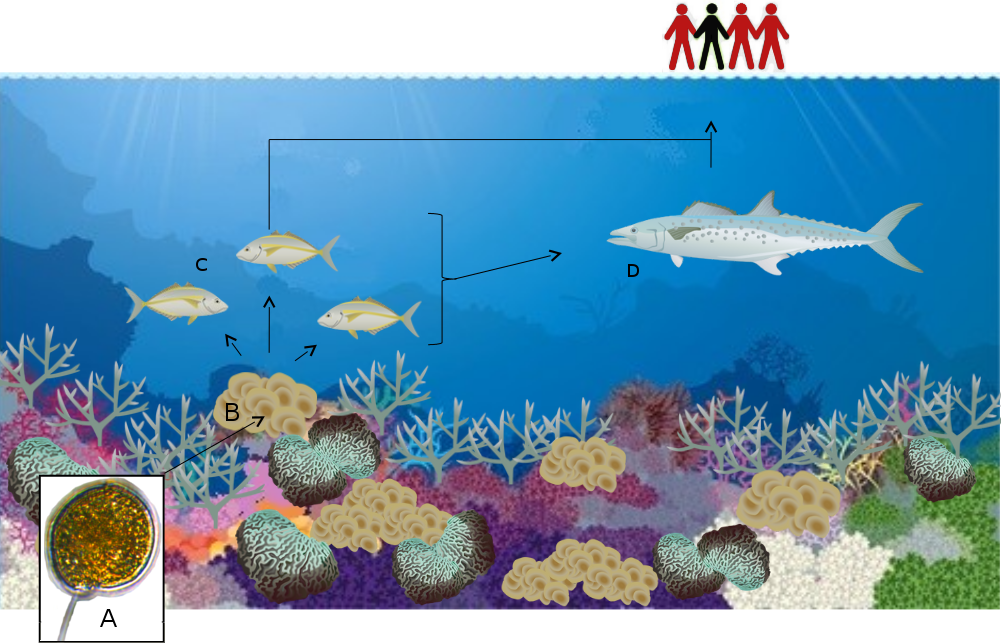
\includegraphics[scale=.55]{Hero_qpcr-figs/CFP-diagram.png} 
\caption{The mechanism of bioaccumulation of CTXs, with \textit{Gambierdiscus} (for example \emph{G. polynesiensis} (A)) at the base of the food web inhabiting the macroalgae \emph{Padina} spp. (B) \cite{padina}. 
A herbivore, here a white trevally (\emph{Pseudocaranx dentex}) (C) \cite{trevally} consumes CTX from \emph{G. polynesiensis} along with the macroalgae, which is then either passes directly to humans through consumption, or through an intermediary piscivorous vector such as Australian spotted mackerel (\emph{Scomberomorus munroi}) (D) \cite{mackerel}. 
Image of \emph{G. polynesiensis} (strain CG15) taken by A. L. Kretzschmar, 2016, Nikon Eclipse TS100 equipped with an Infinite Luminera 1 camera.} 
\label{fig:bioaccom}
\end{figure} 
The symptoms of CFP are largely gastrointestinal and neurotoxic, however, in severe cases, further complications such as cardiovascular or severe neurological symptoms can appear \citep{sims1987theoretical}. 
Species of \emph{Gambierdiscus} spp. are predominantly epiphytic, growing on macroalgae and other substrates such as coral detritus. 
Species of \textit{Gambierdiscus} spp. can vary in the production of ciguatoxins and/or maitotoxins \citep{chinain2010ciguatera,kohli2014high}. 
If a particular \emph{Gambierdiscus} sp. is a CTX producer, and inhabit a palatable macroalgal substrate, the toxins bioaccumulate in herbivorous fish and filter feeders with the potential to travel up the food chain to cause CFP in humans  \citep{chinain1997intraspecific,holmes1998gambierdiscus}. 
\FloatBarrier
\emph{Gambierdiscus} was first identified in 1977, with the type species \emph{G. toxicus} Adachi \& Fukuyo \citep{adachi1979thecal}. 
The genus remained monotypic for 18 years until the discovery of a second species \emph{G. belizeanus} Faust \citep{faust1995observation}. 
To date, the genus comprises 14 described species and 6 ribo/species types
 \citep{smith2016new,fraga2016gambierdiscus,litaker2010global,adachi1979thecal,faust1995observation,chinain1999morphology,litaker2009taxonomy,dai2017taxonomic,nishimura2014morphology,rhodes2017new,kretzschmar2017characterization,fraga2011gambierdiscus,xu2014distribution,fraga2014genus} .
A major revision of the \emph{Gambierdiscus} species taxonomy was undertaken by Litaker et al. (2009). 
Reports of \emph{Gambierdiscus} spp. identified based on morphology alone, prior to this revision; need to be considered with caution as several new \emph{Gambierdiscus} spp. were defined \cite{holmes1990toxicity,holmes1991strain,holmes1994purification}. 
Further, intra-species variation and inter-species similarities can cause misidentification \citep{bravo2014cellular,kretzschmar2017characterization,kohli2014high}. 
Hence, molecular genetic tools are important for determining the distribution and abundance of  \textit{Gambierdiscus} species and assess the risk of CFP in that region \citep{kohli2014high,kretzschmar2017characterization}. \\

\emph{Gambierdiscus} spp. produce a suite of different polyketide compounds - CTX, maitotoxin (MTX), gambierone, gambieric acid and gambierol have been characterised to date \citep{satake1993gambierol,nagai1992gambieric,rodriguez2015gambierone,murata1993structure,murata1989structures}. 
While any of these can contribute to toxicity, only CTX has been clearly linked to CFP in humans \citep{chinain1997intraspecific,holmes1998gambierdiscus}. 
The toxin profile of many \textit{Gambierdiscus} species is not well understood, and many different assays have been used to determine CTX toxicity \citep{globalcig}. 
Assays, such as mouse bioassays and neuroblastoma cell-line bioassays are good indicators of the toxicity of an organism, however species/strain specific toxin profiles needs to be elucidated with LC-MS/MS in order to characterise individual toxin congeners \citep{diogened2014chemistry}. 
The toxin profile of \textit{Gambierdiscus polynesiensis} Chinain \& Faust is one of the only \emph{Gambierdiscus} spp.
whose production of CTX congeners (P-CTX-3B, P-CTX-3C, P-CTX-4A, P-CTX-4B and M-seco-CTX-3C) has been verified by LC-MS/MS in isolates from French Polynesia and the Cook Islands, and is thought to be the principal cause of CFP in the Pacific region \citep{chinain2010growth,rhodes2014production}. 
However recently, a \emph{G. polynesiensis} strain isolated from the Kermandec Islands, Pacific Ocean, did not exhibit CTX toxicity detectable by LC-MS/MS  \citep{rhodes2017epiphytic}.
An uncharacterised peak in the CTX phase of several strains of \emph{Gambierdiscus lapillus} extracts was reported via LC-MS/MS, which did not match any available CTX standards (CTX-3B, CTX-3C, CTX-4A, CTX-4B) \citep{kretzschmar2017characterization}. 
Further, Larsson et al. (2018) found that \emph{G. lapillus} extracts showed ciguatoxin-like activity when investigated with a bioassay. 
Therefore, this species likely produces previously uncharacterised CTX congener(s), and its production of CTX compounds requires further investigation.
Determining the toxin profile of \textit{Gambierdiscus} species requires toxin standards for comparative peak analysis. 
However, these are currently not commercially available. 
Therefore, progress in determining the toxins produced by species of \emph{Gambierdiscus} has been comparatively slow, though bioassays provide a strong indicator for toxin production.\\

CFP was given the "neglected tropical disease" status by a panel of experts co-ordinated by the Intergovernmental Oceanographic Commission’s (IOC) Intergovernmental Panel on Harmful Algal Blooms (IPHAB), as part of the United Nations Educational, Scientific and Cultural Organization), and a global ciguatera strategy was developed \citep{globalcig}. 
One element of the IOC/IPHAB ‘Global Ciguatera Strategy’ is to  investigate various species of the genus \emph{Gambierdiscus}, determine which species produce CTXs through LC-MS/MS and other means, and develop efficient and reliable molecular monitoring tools for the species of interest \citep{globalcig}. 
Quantitative PCR (qPCR) is a useful molecular genetic screening tool, as it can give species-specific and quantitative results from DNA samples extracted from environmental samples \citep{globalcig}. \\
\FloatBarrier
Currently there is one qPCR assay to identify the presence of the genera \emph{Gambierdiscus/Fukuyoa} \citep{smith2017molecular}. 
Assays for species specific identification are available for 9 of the 14 described \emph{Gambierdiscus} spp. and 3 out of 6 undescribed \emph{Gambierdiscus} sp. types/ribotypes (Table ~\ref{tbl:qpcrTable}). 
It is noteworthy that the qPCR assays described by Darius et al. (2017) rely on species identification based on the melt curve of the qPCR product, which requires any subsequent users of these assays to have a reference culture for positive identification rather than rely on a positive result being linked to the species investigated. 
Assays are available for 2 of the 3 species of \emph{Fukuyoa} (Table ~\ref{tbl:qpcrTable}), which seceded from \emph{Gambierdiscus} as their own genus in 2015 \citep{gomez2015fukuyoa}. 
\textit{Fukoyoa} spp. are of interest for monitoring purposes as they produce MTXs, however the involvement of MTXs in CFP has not been resolved yet \citep{kohli2014feeding}.

\begin{table}
\caption{Published qPCR assays for \emph{Gambierdiscus} and \emph{Fukoyoa} spp.}
\label{tbl:qpcrTable}
\begin{tabular}{ | p{6cm} | p{3cm} | p{4cm} | }
\hline
\textbf{Species} & \textbf{Method}& \textbf{Reference} \\
\hline
\multicolumn{3}{| c |}{\textbf{\textit{Gambierdiscus} spp.}}\\
\hline
\emph{G. australes}&TaqMan Probes \& SYBR Green&\citep{nishimura2016quantitative,darius2017tectus}\\
\hline
\textit{G. belizeanus}&SYBR Green&\citep{vandersea2012development}\\
\hline
\textit{G. caribaeus}&SYBR Green&\citep{vandersea2012development}\\
\hline
\emph{G. carolinianus}&SYBR Green&\citep{vandersea2012development}\\
\hline
\textit{G. carpenteri}&SYBR Green&\citep{vandersea2012development}\\
\hline
\emph{G. pacificus}& SYBR Green&\citep{darius2017tectus}\\
\hline
\emph{G. polynesiensis}& SYBR Green&\citep{darius2017tectus}\\
\hline
\emph{G. scabrosus}&TaqMan Probes&\citep{nishimura2016quantitative}\\
\hline
\emph{G. toxicus}& SYBR Green&\citep{darius2017tectus}\\
\hline
\textit{Gambierdiscus} sp. ribotype 2&SYBR Green&\citep{vandersea2012development}\\
\hline
\textit{Gambierdiscus} sp. type 2&TaqMan Probes&\citep{nishimura2016quantitative}\\
\hline
\textit{Gambierdiscus} sp. type 3&TaqMan Probes&\citep{nishimura2016quantitative}\\
\hline
\multicolumn{3}{| c |}{\textbf{\textit{Fukuyoa} spp.}}\\
\hline
\textit{Fukoyoa ruetzleri}&SYBR Green&\citep{vandersea2012development}\\
\hline
\textit{Fukoyoa} cf. \textit{yasumotoi}&TaqMan Probes&\citep{nishimura2016quantitative}\\
\hline
\end{tabular}
\end{table}
\FloatBarrier

In Australia, outbreaks of CFP occur annually in Queensland \citep{qldcig}. 
However, due to the complicated presentation of symptoms, the reporting rate is less than 20\% \citep{lewis2006ciguatera}. 
Annually, there have been 7-69 reported cases between 2011 and 2015 (considering the report rate, $>$ 35-345 cases, see Table ~\ref{tbl:CFPTable}), with 2 fatalities reported in the state \citep{tonge1967ciguatera}. 
Cases of ciguatera from Spanish Mackerel (\textit{Scomberomorus commerson}) caught in NSW have been reported since 2014 \cite{farrellclinical}, with five separate outbreaks affecting a total of 24 people since then \citep{farrell2017management}. 
Farrell et al. (2017) put forward a series if recommendations managing the emerging CFP risk in NSW.

Despite the prevalence of CFP in Australia, the characterization of \textit{Gambierdiscus} species present in Australia is incomplete. 
A species that produces known CTX toxins has not been identified from Australia as yet. 
Larsson et al. (2018) have identified some candidate species, two of which show some CTX-like bioactivity \cite{larsson2018toxicology}.
Over 50\% of Australia's vast coastline (total 66,000 km) is tropical or subtropical, and may be considered potential habitat for \emph{Gambierdiscus} spp. \citep{kretzschmar2017characterization}. 
Seven species of \emph{Gambierdiscus} have been identified from the sub-tropical east Australian coastline namely, \emph{G. belizeanus} \citep{murray2014molecular}, \emph{G. carpenteri} \citep{kohli2014high,sparrow2017effects}, \emph{G. honu} (based on D8-D10 LSU sequence matching to a study by Richlen et al. \cite{richlen2008phylogeography}) \citep{rhodes2017new}, \emph{G. lapillus} \citep{kretzschmar2017characterization,larsson2018toxicology}, \emph{G. toxicus} \citep{hallegraeff2010algae} and two potentially new species \cite{larsson2018toxicology}, as well as \emph{F. yasumotoi}  \citep{murray2014molecular}). 
Using high throughput amplicon sequencing, \textit{Gambierdiscus} was identified to the genus level in Broome, Western Australia \citep{kohli2014cob}, indicating that this is a coastline that should be examined further for CFP risk. 
qPCR primers that can be used for identification in Australia for potential monitoring purposes, have been developed for \emph{G. belizeanus}, \emph{G. carpenteri} and \emph{F. yasumotoi} \citep{nishimura2016quantitative,vandersea2012development}. 
 
\begin{table}
\caption{Cases of Ciguatera Fish Poisoning reported to health authorities in Queensland, Australia, between 2011 and 2015, by Queensland Health \citep{qldcig}.}
\label{tbl:CFPTable}
\begin{tabular}{ | p{6cm} | p{1.5cm} | p{1.5cm}| p{1.5cm} | p{1.5cm} | p{1.5cm} | }
\hline
Year &2011&2012&2013&2014&2015\\
\hline
Recorded CFP cases&18&7&25&69&11\\
\hline
Extrapolated CFP indcidences&$\sim$90&$\sim$35&$\sim$125&$\sim$345&$\sim$55\\
\hline
\end{tabular}
\end{table}
\FloatBarrier

The aim of this study was to develop and test a qPCR assay to detect \emph{G. lapillus} that exclusively amplifies the target species without requiring the operator to have a positive control for comparison. 
The assay was then applied to environmental samples for detection and enumeration of \textit{G. lapillus}.

\section*{Materials and methods}
\subsection*{Clonal strains and culturing conditions}
\FloatBarrier
Three strains of \emph{G. lapillus} and one strain of \emph{G.} cf. \emph{silvae} were isolated from Heron Island, Australia, as previously described \citep{kretzschmar2017characterization}. 
Two strains of \emph{G. polynesiensis} were isolated from Rarotonga, Cook Islands (Table ~\ref{tbl:StrainTable}). 
The cultures were maintained in 5x diluted F/2 media \cite{holmes1991strain} at 27 $^{\circ}$C, 60mol$\bullet$-m$^{2}$ $\bullet$-s light in 12hr light to dark cycles.
\begin{table}  
\caption{List of \emph{Gambierdiscus} clonal strains used for the qPCR assay.}
\label{tbl:StrainTable}
\begin{tabular}{ | p{2cm} | p{2cm} | p{2cm}| p{3cm} | p{3cm} | p{2cm} | }
\hline
\textbf{Species} & \textbf{Collection site} & \textbf{Collection date} &\textbf{Latitude} & \textbf{Longitude} & \textbf{Strain name} \\
\hline
\emph{G. lapillus} &Heron Island, Australia &July 2014 &23$^{\circ}$ 4420' S&151$^{\circ}$ 9140' E & HG4 \\
\hline
&&&&& HG6\\
\hline
&&&& &HG7\\
\hline
%&&&& &HG26\\
%\hline
\emph{G. polynesiensis}&Rarotonga, Cook Islands&November 2014 &21$^{\circ}$ 2486' S&159$^{\circ}$ 7286' W & CG14 \\
\hline
&&&&&CG15\\
\hline
\emph{G.} cf. \emph{silvae}&Heron Island, Australia &July 2014 &23$^{\circ}$ 4420' S&151$^{\circ}$ 9140' E& HG5\\
\hline
\end{tabular}
\end{table}
\FloatBarrier

\subsection*{DNA extraction and species specific primer design}
\FloatBarrier
Genomic DNA was extracted using a modified CTAB method \citep{verma2016molecular}. 
The purity and concentration of the extracted DNA was measured using the Nanodrop (Nanodrop2000, Thermo Scientific), and the integrity of the DNA was visualised on 1\% agarose gel.
A unique primer set was designed for the small-subunit (SSU) rDNA region of \emph{G. lapillus} %and \emph{G. polynesiensis}, 
based on sequences available in the GenBank reference database (    KU558929-33). 
The target sequences were aligned against sequences of all other \emph{Gambierdiscus} spp. that were available on GenBank reference database, with the MUSCLE algorithm (maximum of 8 iterations) \citep{edgar2004muscle} used through the Geneious software, version 8.1.7 \citep{kearse2012geneious}. 
Unique sites were determined manually (Table ~\ref{tbl:PrimerTable}). 
Primers were synthesised by Integrated DNA Technologies (IA, USA).
The primer set was tested systematically for secondary product formation for all 3 strains of \emph{G. lapillus} (Table ~\ref{tbl:StrainTable}) via standard PCR in 25$\mu$l mixture in PCR tubes.
The mixture contained 0.6 $\mu$M forward and reverse primer, 0.4 $\mu$M BSA, 2 - 20 ng DNA, 12.5 $\mu$l 2xEconoTaq (Lucigen) and 7.5 $\mu$l PCR grade water.
The PCR cycling comprised of an initial 10 min step at 94 $^{\circ}$C, followed by 30 cycles of denaturing at 94 $^{\circ}$C for 30 sec, annealing at 60 $^{\circ}$C for 30 sec and extension at 72 $^{\circ}$C for 1 min, finalised with 3 minutes of extension at 72 $^{\circ}$C. 
Products were visualised on a 1\% agarose gel.
\begin{table}
\caption{G. lapillus specific qPCR primer set for SSU rDNA designed in this study.}
\label{tbl:PrimerTable}
\begin{tabular}{ | p{2.5cm} | p{2cm} | p{2cm} | p{6.5cm} | }
\hline
\textbf{Primer name} &\textbf{Amplicon size} &  \textbf{Synthesis direction of primer} & \textbf{Sequence (5'-3')} \\
\hline
qGlapSSU2F&138bp&Forward&TTTTTGTCCCAGGAGGGTGA\\
\hline
qGlapSSU2R&&Reverse&TGAGGCCAAAACTCGAAAATC\\
\hline
%\emph{G. polynesiensis}&208bp&qGpolySSU2F&Forward&TGGAGCGGAGATATAGCAGA\\
%\hline
%& &qGpolySSU2R&Reverse&CACCCGATCTCTAGTTGGCAT\\
%\hline
\end{tabular}
\end{table}
\FloatBarrier

\subsection*{Evaluation of primer specificity}
To verify primer set specificity as listed in Table ~\ref{tbl:PrimerTable}, DNA was extracted using CTAB buffer \cite{zhou1999analysis} from \emph{G. australes} (CCMP1650 and CG61), \emph{G. belizeanus} (CCMP401), \emph{G. carpenteri} (UTSMER9A3), \emph{G. pacificus} (CAWD149) and \emph{G.} cf. \emph{silvae} (HG5). 
\emph{G. cheloniae} (CAWD232) DNA was extracted using a PowerSoil™ DNA isolation kit (Mo Bio Inc., CA, USA). 
\emph{G. scabrosus} (KW070922\_1) DNA was extracted using DNeasy Plant Mini Kit (Quiagen, Tokyo, Japan) according to the manufacturer's protocol. 
For all extracted samples, the presence and integrity of genomic DNA was assessed on 1\% agarose gel. 
The primer set designed for \emph{G. lapillus} was tested for cross-reactivity against all other \emph{Gambierdiscus} spp. available via PCR (BioRadT100 Thermal Cycler (CA, USA)), appropriate positive and negative controls were applied. 
PCR amplicons were visually assessed on 1\% agarose gel.


\subsection*{Evaluation of primer sensitivity}
The qPCR reaction mixture contained 10 $\mu$l SYBR Select Master Mix (Thermo Fisher Scientific), 7 $\mu$l MilliQ water, 0.5 $\mu$M forward and reverse primers and 2 - 20 ng DNA template, for a final volume of 20 $\mu$l. 
Cycling conditions consisted of 10 min at 95, then 40 cycles of 95 $^{\circ}$C for 15 seconds and 60 $^{\circ}$C for 30 seconds, followed by a temperature gradient for melt curve construction.
\subsection*{Calibration curve construction}
Standard curves were constructed to determine the efficiency of the assay, using a synthetic gene fragment approach, and also to use to quantify species presence, using calibration curves based on DNA extracted from known cell numbers. 
For curves based on synthetic gene fragments, a 10-fold serial dilution of a synthesised fragment containing the SSU target sequence, forward and reverse primer sites and 50bp flanking both primer sites matching sequencing results were generated. 
Cell-based standard curves were constructed using 10-fold dilutions of gDNA extract of known cell concentrations.
The calibration curves for both methods were calculated (R$^{2}$, PCR efficiency and regression line slope) and graphed in R version 3.2.3 \citep{rlang}, using R studio version 1.0.136 \citep{rstudio} and the ggplot2 package \citep{ggplot2}. 

\subsubsection*{Gene based calibration curve}
For the target amplicons of \emph{G. lapillus}, a DNA fragment spanning the target sequence, the reverse and forward primer sites and an extra 50bp on either end was synthesised called gBlocks \textsuperscript{\textregistered} by Integrated DNA Technologies (IDT, IA, USA). 
Lyophilized gBlocks \textsuperscript{\textregistered} was re-suspended in 1x TE (Tris 1M, EDTA 0.5 pH8) to a concentration of 1 ng/$\mu$l. 
The copy number of gene fragment was then calculated as 2.88x10$^{10}$ for \textit{G. lapillus}. 
The stock solution was serially diluted (10-fold) and dilutions between 10$^{3}$ and 10$^{8}$ were amplified by qPCR (on StepOnePlus System by Applied Biosystems (Thermo Fisher Scientific, Waltham, MA, USA) in triplicate.

\subsubsection*{Cell based calibration curve}
Two strains of \emph{G. lapillus} (HG4 and HG7) were used to construct cell based standard curves. 
Cells were counted under a Nikon Eclipse TS100 (Australia) microscope using a Sedgwick Rafter counting chamber. 
DNA was extracted with the FastDNA spin kit for soil by MP Biomedicals (CA, USA), as per the manufacturer's instructions. 
The gDNA extracts were 10-fold serially diluted. 
Dilutions ranging from 3880 to 0.04 cells and 5328 to 0.05 for HG4 and HG7 respectively.  
Samples were amplified via qPCR (on StepOnePlus System by Applied Biosystems (Thermo Fisher Scientific, Waltham, MA, USA) in triplicate.

\subsection*{Determination of extractable gene copies per cell for \emph{G. lapullis}}

To determine the extractable mean SSU rDNA copies per cell, the known cell counts for the cell based calibration curve were used as input for calculation. 
Copy number was defined as a linear regression of the gene based calibration curve using the input cell counts to determine extractable SSU rDNA copy number per cell.

\subsection*{Screening environmental samples for \emph{G. lapillus}}
\FloatBarrier
Around Heron Reef (Fig. ~\ref{fig:samplesites}) 25 sites (within 1km of the shore) were sampled in October 2015, in spatial replicates (A, B, C) within a 2m radius. 
Representatives of three genera of macroalgae that commonly grow on this reef, \textit{Chnoospora} spp, \textit{Padina} sp. and \textit{Saragassum} sp., were sampled for the presence of epiphytic \emph{Gambierdiscus} spp. For each sample, about 200 g of macroalgae was collected from approximately 1 m deep water at low tide and briefly placed in plastic bags containing 200 to 300 ml of ambient seawater. 
They were shaken vigorously for 5 min to detach the epiphytic dinoflagellates from the macroalgae. 
This seawater was passed through $>$ 120 μm mesh filter to remove any remaining larger fauna and debris. 
The collected seawater was centrifuged at 1000 rpm. The supernatant was discarded and the pellet was dissolved in 10 ml RNAlater (Ambion®, Austin, TX, USA) for preservation and stored at 4$^{\circ}$C.
Samples were screened in triplicate for both \emph{G. lapillus} on a StepOnePlus System by Applied Biosystems (Thermo Fisher Scientific, Waltham, MA, USA).
\begin{figure} 
%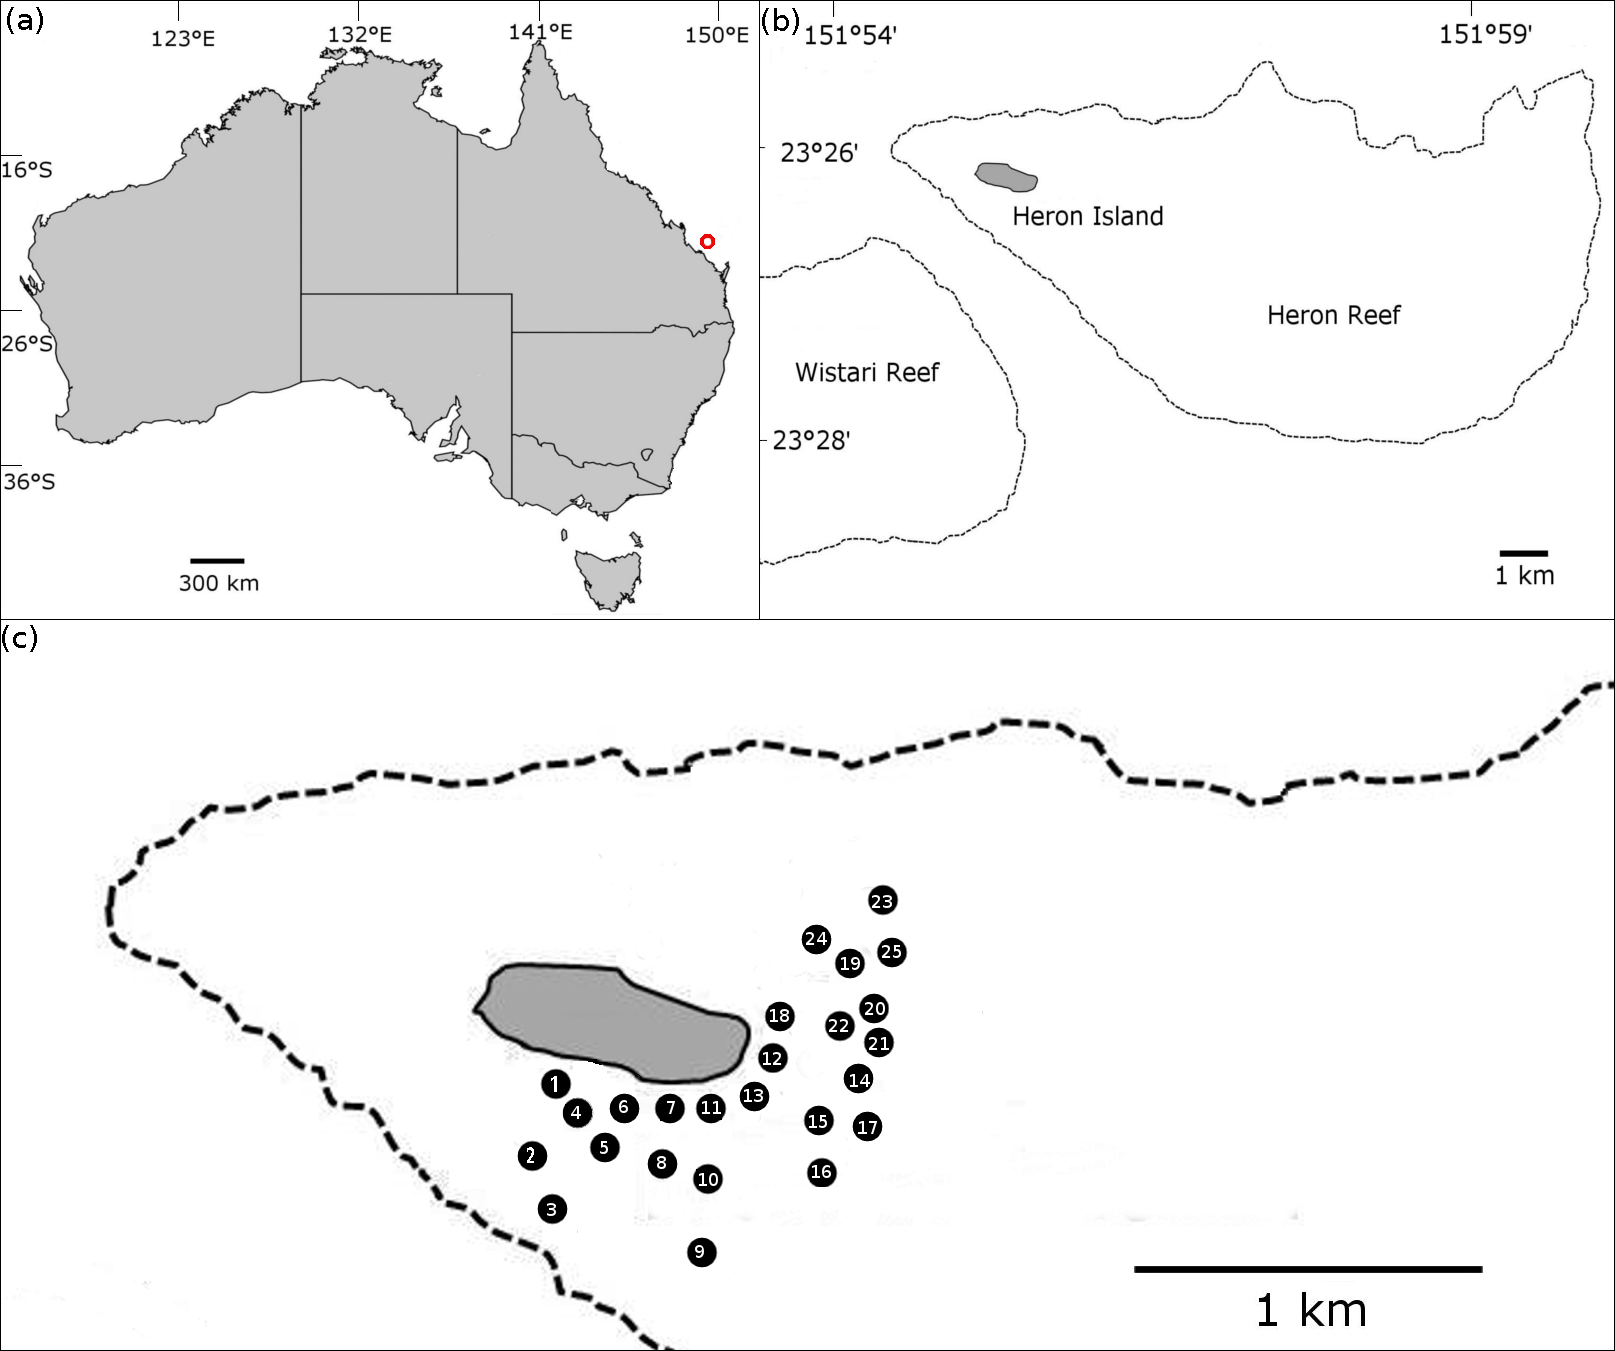
\includegraphics[scale=1.7]{Hero_qpcr-figs/Fig1_Heron_sample-map_Dec18.png} 
\caption{(A) Map of Australia, with the position of Heron Island (red circle); (B) Heron Island including surrounding reefs; (C) Approximate location of sampling sites around Heron Island.} 
\label{fig:samplesites}
\end{figure} 


\section*{Results}
% Place tables after the first paragraph in which they are cited.
\begin{table}[!ht]
\begin{adjustwidth}{-2.25in}{0in} % Comment out/remove adjustwidth environment if table fits in text column.
\centering
\caption{
{\bf Table caption Nulla mi mi, venenatis sed ipsum varius, volutpat euismod diam.}}
\begin{tabular}{|l+l|l|l|l|l|l|l|}
\hline
\multicolumn{4}{|l|}{\bf Heading1} & \multicolumn{4}{|l|}{\bf Heading2}\\ \thickhline
$cell1 row1$ & cell2 row 1 & cell3 row 1 & cell4 row 1 & cell5 row 1 & cell6 row 1 & cell7 row 1 & cell8 row 1\\ \hline
$cell1 row2$ & cell2 row 2 & cell3 row 2 & cell4 row 2 & cell5 row 2 & cell6 row 2 & cell7 row 2 & cell8 row 2\\ \hline
$cell1 row3$ & cell2 row 3 & cell3 row 3 & cell4 row 3 & cell5 row 3 & cell6 row 3 & cell7 row 3 & cell8 row 3\\ \hline
\end{tabular}
\begin{flushleft} Table notes Phasellus venenatis, tortor nec vestibulum mattis, massa tortor interdum felis, nec pellentesque metus tortor nec nisl. Ut ornare mauris tellus, vel dapibus arcu suscipit sed.
\end{flushleft}
\label{table1}
\end{adjustwidth}
\end{table}

\subsection*{Evaluation of primer specificity}
\FloatBarrier
The qGlapSSU2F - qGlapSSU2R primer pair (Table ~\ref{tbl:PrimerTable}) produced an amplified product of 138 bp for all five strains of \emph{G. lapillus}, while no amplification was observed for genetically closely related species \emph{G. belizeanus}, \emph{G. cheloniae}, \emph{G. pacificus} and \emph{G. scabrosus}. 
Other species of \emph{Gambierdiscus} from different clades, \emph{G. australes}, \emph{G. carpenteri}, \emph{G. polynesiensis} and \emph{G.} cf. \emph{silvae} (Table ~\ref{tbl:CrossreactTable}) were also not amplified using this primer set \citep{smith2016new,kretzschmar2017characterization}.

\begin{table}
\caption{Cross-reactivity of the qPCR primer set based on presence absence of PCR product visualised in agarose gel.}
\label{tbl:CrossreactTable}
\begin{tabular}{ | p{4cm} | p{3cm} | p{2cm} | p{2.5cm} | }% p{2.5cm} | }
\hline
\textbf{Template} & \textbf{Strain name} & \textbf{gDNA gel band} & \textbf{GlapSSU2F-GlapSSU2R} \\
\hline
\emph{G. australes} & CCMP1650 &+&-\\
\hline
& CG61 &+&-\\
\hline
\emph{G. belizeanus}&CCMP401&+&-\\
\hline
\emph{G. carpenteri}&UTSMER9A3&+&-\\
\hline
\emph{G.cheloniae}&CAWD232&+&-\\
\hline
\emph{G. lapillus}&HG1&+&+\\
\hline
&HG4&+&+\\
\hline
&HG6&+&+\\
\hline
&HG7&+&+\\
\hline
&HG26&+&+\\
\hline
\emph{G. pacificus}&CAWD149&+&-\\
\hline
\emph{G. polynesiensis}&CG14&+&-\\
\hline
&CG15&+&-\\
\hline
\emph{G. scabrosus}&KW070922\_1&+&-\\
\hline
\emph{G.} cf. \emph{silvae}&HG5&+&-\\
\hline
\end{tabular}
\end{table}
\FloatBarrier

\subsection*{Evaluation of primer sensitivity}
\FloatBarrier
The cell-based standard curves for \emph{G. lapillus} (HG4 and HG7, Fig. ~\ref{fig:stdCurve}a) showed high linearity with R$^{2}$ approaching 1.00. 
The slope for the Ct vs. log$_{10}$ cell for HG4  was -3.4, which corresponds to an efficiency 96.8 \%; and -3.51, which corresponds to an efficiency of 92.7 \% for HG7 (Fig. ~\ref{fig:stdCurve}). 
The linear detection for both \emph{G. lapillus} isolates covered six orders of magnitude. 
The lowest number of cells detected were 0.04 and 0.05 cells for HG4 and HG7 respectively (Fig. ~\ref{fig:stdCurve}a).
\begin{figure}
%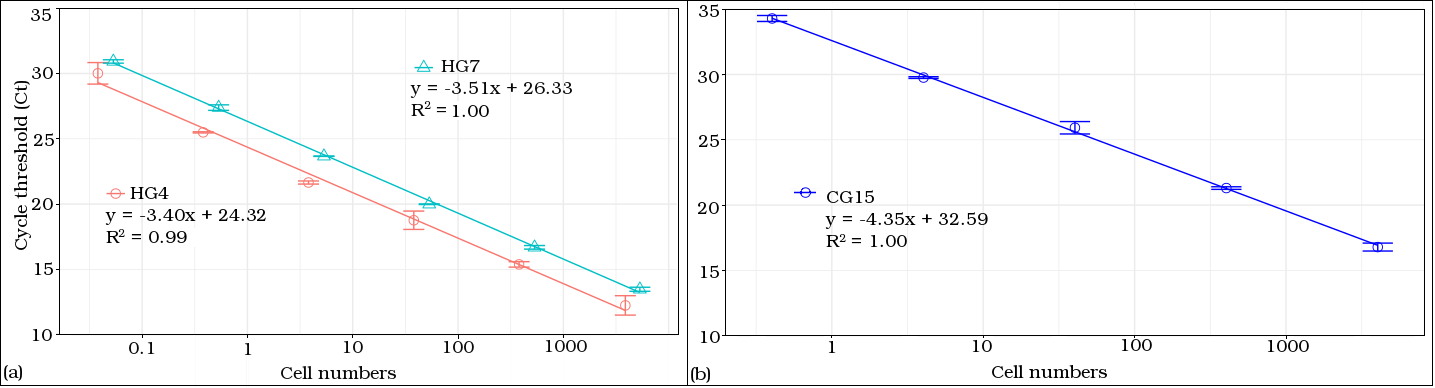
\includegraphics[scale=.85]{Hero_qpcr-figs/Fig2_cell-based-stds-merged.png}
\caption{qPCR cell based standard curves of \emph{G. lapillus} strains HG4 (circle) and HG7 (triangle). Error bars represent the deviation of technical replicates during reactions.}
\label{fig:stdCurve}
\end{figure}



The gene based (gBlocks) standard curve for \emph{G. lapillus} covered linear detection over 7 orders of magnitude, with a slope of -3.42, and a PCR efficiency of 96 \% (Fig. ~\ref{fig:lapigblocks}). 
The detection limit tested was less than 10$^{5}$ gene copy numbers. 
The Ct for the lowest gene copy number tested was less than 25, so it is likely that the sensitivity is lower than 10$^{5}$ gene copy numbers (Fig. ~\ref{fig:lapigblocks}).\\
\begin{figure}
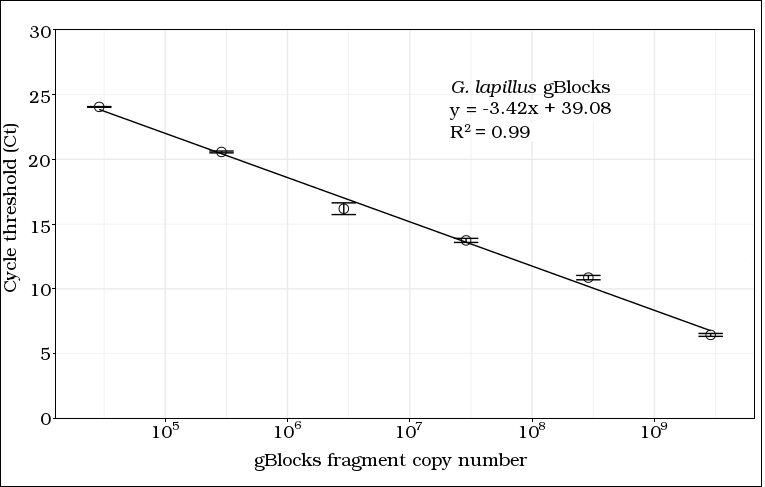
\includegraphics[scale=.8]{Hero_qpcr-figs/Fig3_gblocks-standards.png}
\caption{qPCR gene based standard curves of \emph{G. lapillus}. Error bars represent the deviation of technical replicates during reactions.}% and (B) \emph{G. polynesiensis}.} 
\label{fig:lapigblocks}
\end{figure}
\FloatBarrier

\FloatBarrier


\subsection*{Quantification of extractable SSU rDNA copy number per cell of \emph{G. lapillus}}
The detectable SSU copies for \emph{G.lapillus} were 2.24x10$^{4}$ and 5.85x10$^{3}$ copies per cell for HG4 and HG7 respectively. 

\subsection*{Screening environmental samples for \emph{G. lapillus} abundance }
\FloatBarrier
To evaluate the adequacy of the \emph{G. lapillus} 
qPCR assay for environmental screening, the assay was applied to environmental community DNA extracts collected around Heron Island (Fig. ~\ref{fig:samplesites}). 
A relatively low cell abundance was detectable for \emph{G. lapillus}. 
Ct values for \emph{G. lapillus} detection in environmental samples were calibrated to the HG7 standard curve and calculated as cells.g$^{-1}$ wet weight macroalgae (Table ~\ref{tbl:MacroalgaeTable}).  
\emph{G. lapillus} was detected across 24 of the 25 sampling sites. 
At sites at which \textit{G. lapillus} was present, it showed a patchy distribution, being present at two of the three spatial replicates in the majority of samples (17 of 25 sample sites), followed by all three spatial replicates testing positive (6 out of 25 sites) and at one site only one of the spatial replicates was positive (Fig. ~\ref{fig:envposneg}). \\
\emph{G. lapillus} was detected at 71 out of the 75 spatial replicates, specifically at 24/32, 22/33 and 8/10 samples from \emph{Chnoospora} sp., \emph{Padina} sp. and \emph{Saragassum} sp. as substrate respectively (Table ~\ref{tbl:MacroalgaeTable}).
Patchiness was also found in the abundance as well as the distribution of \emph{G. lapillus}, from 0.24 cells.g$^{-1}$ wet weight macroalgae to 49.51 cells.g$^{-1}$ wet weight macroalgae, with a mean of 5.84 cells.g$^{-1}$ wet weight macroalgae. 
For example (4A - \emph{Chnoospora} sp.) and (4B - \emph{Padina} sp.) hosted comparable cell numbers (1.12 cells and 1.65 cells.g$^{-1}$ wet weight algae respectively) while no \emph{G. lapillus} cells were detected on (4C - \emph{Padina} sp.).
Only at one of 25 sampling sites, no \emph{G. lapillus} presence was detected across all three spatial replicates (19A, B, C).
At all other sites, the presence of \textit{G. lapillus} varied between spatial replicates but did not significantly differ between macroalgal host or location (Fig. ~\ref{fig:envHG7}). 

\begin{longtable}{ | p{2cm} | p{2cm} | p{3cm} | p{3.5cm} |}
\caption{Screening of macroalgal samples for \emph{G. lapillus} and cell density estimates via qPCR. Cell numbers were modeled on the type strain HG7. N/D denotes not detected; N/A denotes not attempted due to loss of sample.}\\
\hline
\label{tbl:MacroalgaeTable}
\textbf{Sample ID}&\textbf{Spatial replicate}&\textbf{Macroalgal substrate}&\textbf{\textit{G. lapillus} cell number}\\
\hline
1&A&\emph{Padina} sp.&N/D\\
\hline
1&B&\emph{Sargassum} sp.&10.55
\\
\hline
1&C&\emph{Padina} sp.&2.75
\\
\hline
2&A&\emph{Padina} sp.&N/D\\
\hline
2&B&\emph{Padina} sp. 
&4.33\\
\hline
2&C&\emph{Padina} sp.&4.27\\
\hline
3&A&\emph{Padina} sp. %\& \emph{Chnoospora} sp.
&6.13 %ex4
\\
\hline
3&B&\emph{Chnoospora sp.}&0.62
\\
\hline
3&C&\emph{Padina} sp. 
&N/D\\
\hline
4&A&\emph{Chnoospora} sp.&1.12 
\\
\hline
4&B&\emph{Padina} sp.&1.65
\\
\hline
4&C&\emph{Padina} sp.&N/D\\
\hline
5
&A&\emph{Padina} sp.&9.35\\
\hline
5
&B&\emph{Padina} sp.&N/D\\
\hline
5
&C&\emph{Padina} sp.&N/D\\
\hline
6&A& 
\emph{Chnoospora} sp.&N/D\\
\hline
6&B&\emph{Padina} sp.&1.69
\\
\hline
6&C&\emph{Padina} sp.&1.92
\\
\hline
7  
&A&
\emph{Padina} sp. 
&N/D\\
\hline
7 
&B&\emph{Padina} sp. 
&0.26\\
\hline
7 
&C&\emph{Padina} sp. 
&1.29\\
\hline
8&A&\emph{Chnoospora} sp.&N/D\\ 
\hline
8&B&\emph{Chnoospora} sp.&17.09
\\
\hline
8&C&\emph{Chnoospora} sp.&4.27
\\
\hline
9&A&\emph{Chnoospora} sp.&N/D\\
\hline
9&B&\emph{Padina} sp. 
&49.51
\\
\hline
9&C&\emph{Padina} sp. 
&18.58 
\\
\hline
10&A&\emph{Padina} sp. 
&0.91
\\
\hline
10&B&\emph{Padina} sp. 
&N/D\\
\hline
10&C&\emph{Chnoospora} sp.&5.95
\\
\hline
11&A&\emph{Padina} sp. 
&2.01 %ex15
\\
\hline
11&B&\emph{Chnoospora} sp.&4.89
\\
\hline
11&C&\emph{Chnoospora} sp.&N/D\\
\hline
12&A&\emph{Chnoospora} sp.&6.70\\
\hline
12&B&\emph{Chnoospora} sp.&8.83
\\
\hline
12&C&\emph{Chnoospora} sp.&3.08
\\
\hline
13&A&\emph{Chnoospora} sp.&2.58 
\\
\hline
13&B&\emph{Chnoospora} sp.&9.39
\\
\hline
13&C& 
\emph{Chnoospora} sp.&N/D\\
\hline
14&A&\emph{Chnoospora }sp.&0.02
\\
\hline
14&B&\emph{Chnoospora} sp.&N/D\\
\hline
14&C&\emph{Chnoospora }sp.&9.24
\\
\hline
15&A&\emph{Chnoospora }sp.&5.27
\\
\hline
15&B&\emph{Padina} sp. 
&48.46
\\
\hline
15&C&\emph{Padina} sp.
&2.71
\\
\hline
16&A&
\emph{Chnoospora }sp.&2.81
\\
\hline
16&B& 
\emph{Chnoospora }sp.&10.26
\\
\hline
16&C&\emph{Chnoospora }sp.&N/D\\
\hline
17&A& 
\emph{Chnoospora} sp.&5.50
\\
\hline
17&B&\emph{Chnoospora }sp.&1.23
\\
\hline
17&C&\emph{Padina} sp.&10.32
\\
\hline
18&A&\emph{Chnoospora }sp.&N/D\\
\hline
18&B&\emph{Chnoospora} sp.&37.68
\\
\hline
18&C&\emph{Chnoospora} sp.&5.57
\\
\hline
19&A&\emph{Padina} sp.&N/D\\
\hline
19&B&\emph{Padina} sp.&N/D\\
\hline
19&C&\emph{Padina} sp.&N/D\\
\hline
20
&A&\emph{Sargassum} sp.&N/D\\
\hline
20
&B&\emph{Sargassum} sp.&0.19\\
\hline
20
&C&\emph{Sargassum} sp.&0.18\\
\hline
21
&A&\emph{Sargassum} sp.&N/D\\
\hline
21
&B&\emph{Sargassum} sp.&2.11\\
\hline
21
&C&\emph{Sargassum} sp.&2.05\\
\hline
22
&A&\emph{Padina} sp.&7.17\\
\hline
22
&B&\emph{Padina} sp.&2.67\\
\hline
22
&C&\emph{Padina} sp.&8.64\\
\hline
23&A&\emph{Chnoospora }sp.&1.24
\\
\hline
23&B&\emph{Chnoospora }sp.&5.90
\\
\hline
23&C&\emph{Chnoospora} sp.&N/D\\
\hline
24&A&\emph{Sargassum} sp.&1.91
\\
\hline
24&B&\emph{Sargassum} sp.&2.90
\\
\hline
24&C&\emph{Sargassum} sp.&3.97
\\
\hline
25&A&\emph{Padina} sp.
&2.24
\\
\hline
25&B&\emph{Chnoospora }sp.
&1.36
\\
\hline
25&C&\emph{Padina} sp.
&2.00
\\
\hline
\end{longtable}
\FloatBarrier
\begin{figure} 
%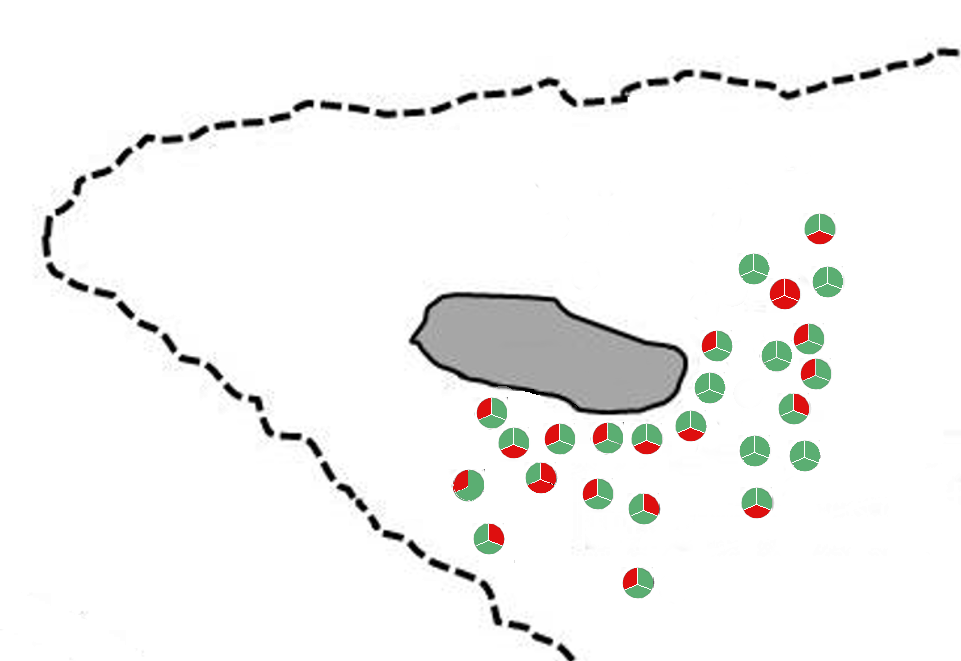
\includegraphics[scale=2.5]{Hero_qpcr-figs/Fig4_Heron-positive-negative-samplingsites_Dec18.png} 
\caption{\emph{G. lapillus} presence at the macroalgal sampling sites around Heron Island. The spatial replicates for each site are set up as shown in (A); the sites in (B) linked to numbering in Fig. ~\ref{fig:samplesites} where positive (green) and negative (red) as per Table ~\ref{tbl:MacroalgaeTable}.} 
\label{fig:envposneg}
\end{figure} 
 
\begin{figure} 
%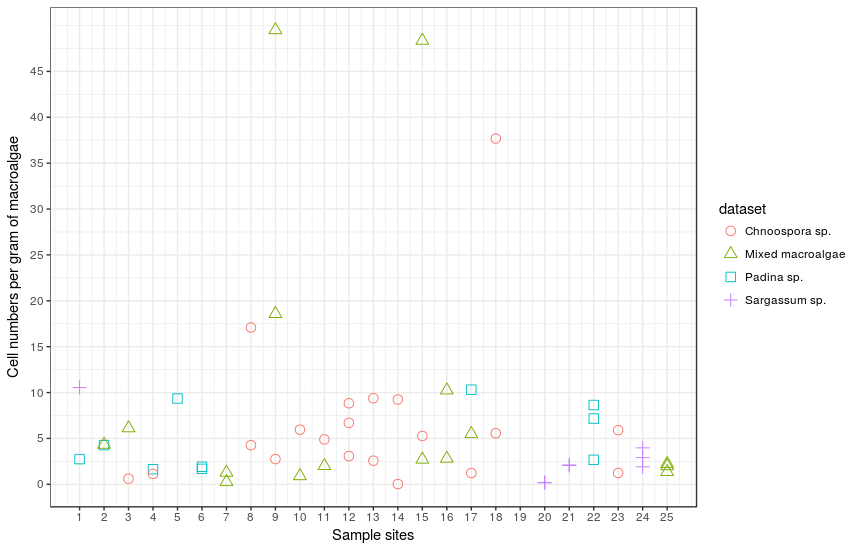
\includegraphics[scale=.75]{Hero_qpcr-figs/Fig5_Env-plot_Nov18.png}
\caption{Detection of \emph{G. lapillus} per spatial replicate at each macroalgal sampling site. Cell numbers were normalised to the HG7 standard curve (Fig. ~\ref{fig:stdCurve}A). Figure also shows spatial replicates per macroalgal substrate where \emph{Chnoospora} sp. samples are represented by circles, \emph{Padina} sp. by squares and \textit{Sargassum} by crosses (Table ~\ref{tbl:MacroalgaeTable}).} 
\label{fig:envHG7}
\end{figure} 
\FloatBarrier

\section*{Discussion}
The aim of the study was to design and validate a species-specific qPCR assay to quantify \emph{G. lapillus} %and \emph{G. polynesiensis}, 
a species that may produce CTX- like toxicity in the Australian GBR region. 
Species-specific PCR primers with high specificity and sensitivity were developed and the SSU copy number for two strains were determined, and were found to differ from one another considerably, as one strain had more than four times the number of genomic rDNA copies. 
We also established that this primer set were effective in measuring the abundance and distribution of \textit{G. lapillus} at the Heron Island reef.
The cross-reactivity of primers designed in this study showed high specificity for both \emph{G. lapillus} while not amplifying when tested against other \emph{Gambierdiscus} spp. 
The species tested for cross-reactivity were chosen because they represented species that are genetically most similar to each target species for the SSU region (as per Fig. 2 in \citep{kretzschmar2017characterization}).
Standard curves were constructed for two strains of \emph{G. lapillus} for which the primers showed high linearity and amplification efficiency (Fig. ~\ref{fig:stdCurve}). 
Hence, this primer set is an accurate and reproducible molecular tool to enumerate the target species exclusively from environmental community DNA extracts. 
More importantly, this assay does not require the operator to rely on melt curves to identify species, or to have access to \emph{G. lapillus} DNA extracts as a positive control. 
Due to the potential CTX production of \emph{G. lapillus} \citep{kretzschmar2017characterization,larsson2018toxicology} the presence and distribution of this species is of interest in Australia where the causative organism(s) for CFP is yet to be established.\\

As CFP risk is linked to the abundance of \emph{Gambierdiscus} species producing CTXs \cite{globalcig,berdalet2012global}, it was important to establish a quantitative assay for detection.
We validated a synthetic gene fragment standard curve of the target region (gBlocks \textsuperscript{\textregistered}) and compared this to cell standard curves to establish an 'absolute' qPCR assay \citep{nishimura2016quantitative,hariganeya2013quantitative}. 
Further, we determined the extractable copy SSU rDNA number for two strains of \emph{G. lapillus} (HG4 and HG7). 
The copy number for \emph{G. lapillus} (5,855.3 to 22,430.3 rDNA copies per cell) were comparable to the copy numbers determined by Vandersea et al. (2012), which ranged from 690 rDNA copies for \emph{G. belizeanus} to 21,498 copies for \emph{G. caribaeus}. 
In comparison, the cell copy numbers determined by Nishimura et al. (2016) ranged from 532,000 copies for \emph{G. scabrosus} and 2,261,000 for \emph{G.} sp. type 3. While the difference in rDNA copy numbers may be due to inter-species differences, or even intra-species as per the \emph{G. lapillus} results, Nishimura et al. (2016) argue that the difference could be underestimation of rDNA copy numbers due to 'ghost' cells counted for total cell number which do not contribute to amplification \citep{nishimura2016quantitative,hariganeya2013quantitative}.
The difference in extractable SSU rDNA copies between the two strains of \emph{G. lapillus} isolated from the same region highlights the importance of carefully verifying qPCR assays based on rRNA genes using multiple local strains.  
A difference of this magnitude may lead to considerably different abundance estimates of \textit{G. lapillus}. 
As the variation between the two strains tested is within the observed variation reported by Nishimura et al. (2016) from single cell qPCR experiments for rDNA copy number elucidation, the difference reported here is likely representative of biological intra-strain variation rather than methodological artifacts. 
A 5-fold difference in toxicity between the same HG4 and HG7 strains for \emph{G. lapillus} was also reported by Kretzschmar et al. (2017), and there was a noticeable difference in growth rate between the two strains observed (but not quantified) in this study. 
The mounting evidence of intra-strain variability in toxicity, detectable rDNA copy numbers and potentially growth rate could have severe implications for qPCR based cell enumeration of environmental samples when attempting to extrapolate CFP risk and requires further investigation.\\
The qPCR assay was successfully tested on environmental DNA extracts from around Heron Island, and gave some insight into \emph{G. lapillus} distribution and abundance. 
The qPCR assay detected \emph{G. lapillus} at all of the sites tested (Fig. ~\ref{fig:envposneg}). 
Within the spatial replicates, the distribution of \emph{G. lapillus} was patchy, as 24 of the 25 sites included at least one replicate with no \textit{G. lapillus} present (Fig. ~\ref{fig:envposneg}). 
Patchiness in the distribution of \textit{Gambierdiscus} species has previously been found in a study of 7 \emph{Bryothamnion} macroalgae spaced 5 to 10 cm apart, in which 5 to 70 cells g-1 algae were found \citep{taylor1986underwater}.\\
%do damn stats
There was no significant difference in the presence/absence of \emph{G. lapillus} cells observed as per the macroalgal host, \emph{Padina} sp. or \emph{Sargassum} sp.\\
Motile behaviour has been observed previously in the field at various time points \citep{yasumoto1977finding,bomber1987ecology}. 
Parsons et al. (2011) reported \emph{Gambierdiscus} sp. behaviour as facultative epiphytes during lab scale experiments, as cells showed attachment as well as motile stages over time in the presence of different macroalgae \citep{parsons2011examination}. 
Taylor \& Gustavson (1983) reported that \emph{Gambierdiscus} cells were captured in plankton tows by de Silva in 1956 but reported as \emph{Goniodoma} \citep{taylor1986underwater}.
Motility could be a factor for the patchy distribution observed in the spatial replicates. 
Across spatial replicates where \emph{G. lapillus} was detected, cell densities were consistent (Fig. ~\ref{fig:envHG7}). 
The average cell density of \emph{G. lapillus} 5.84 cells.g$^{-1}$ wet weight macroalgae, which is comparable to the cell densities recorded by Nishimura et al. (2016) in their environmental screening (Table 4 in \citep{nishimura2016quantitative}).\\

As many authors have pointed out (e.g. \citep{litaker2010global,bomber1989epiphytism,tester2014sampling,cruz2006macroalgal,parsons2011examination,globalcig,lobel1988assessment}), there are several difficulties in determining precise quantification of \textit{Gambierdiscus} species on macroalgae in order to assess potential CFP risk. 
Due to the difference in habitable surface area between samples taken from structurally diverse macroalgae, including those sampled in this study (\emph{Chnoospora}, \emph{Padina} sp. and \emph{Sargassum} sp.), the potential habitable space is difficult to compare. 
Further, in order to assess CFP risk in a given area, the properties of the macroalgae with \emph{Gambierdiscus} spp. epiphytes need to be considered. 
If the macroalgae is structurally or chemically defended against herbivory, any CTX produced by the epiphytes is unlikely to enter the food chain and cause CFP \citep{cruz2006macroalgal}. 
Due to the difficulty in quantifying \emph{Gambierdiscus} spp. on a particular substrate, Tester et al. (2014) proposed have the use of an artificial substrate (commonly available black fibreglass screen of a known surface area) and a standardised sampling method \citep{tester2014sampling}.

\section*{Conclusion}

The qPCR assay developed in this study is an accurate molecular tools to detect and enumerate the presence of \emph{G. lapillus}
in environmental samples. 
The assay was shown to be highly sensitive and accurately detected 0.05 to over 4000 cells for \emph{G. lapillus}. 
Although the toxin profile of \emph{G. lapillus} has not been completely defined, it may produce uncharacterised CTXs congeners \cite{kretzschmar2017characterization,larsson2018toxicology} and therefore is a part of the ciguateric web in Australia.
The assay was applied to spatial replicates from 25 sites around Heron Island on the GBR, which found that \textit{G. lapillus} was commonly present, but had a patchy spatial distribution and abundance. 
The development and validation of a quantitative monitoring tool presented here for \textit{G. lapillus} is in line with Element 1 of the Global Ciguatera Strategy \cite{globalcig}.

\section*{Supporting information}

% Include only the SI item label in the paragraph heading. Use the \nameref{label} command to cite SI items in the text.
\paragraph*{S1 Fig.}
\label{S1_Fig}
{\bf Bold the title sentence.} Add descriptive text after the title of the item (optional).

\paragraph*{S2 Fig.}
\label{S2_Fig}
{\bf Lorem ipsum.} Maecenas convallis mauris sit amet sem ultrices gravida. Etiam eget sapien nibh. Sed ac ipsum eget enim egestas ullamcorper nec euismod ligula. Curabitur fringilla pulvinar lectus consectetur pellentesque.

\paragraph*{S1 File.}
\label{S1_File}
{\bf Lorem ipsum.}  Maecenas convallis mauris sit amet sem ultrices gravida. Etiam eget sapien nibh. Sed ac ipsum eget enim egestas ullamcorper nec euismod ligula. Curabitur fringilla pulvinar lectus consectetur pellentesque.

\paragraph*{S1 Video.}
\label{S1_Video}
{\bf Lorem ipsum.}  Maecenas convallis mauris sit amet sem ultrices gravida. Etiam eget sapien nibh. Sed ac ipsum eget enim egestas ullamcorper nec euismod ligula. Curabitur fringilla pulvinar lectus consectetur pellentesque.

\paragraph*{S1 Appendix.}
\label{S1_Appendix}
{\bf Lorem ipsum.} Maecenas convallis mauris sit amet sem ultrices gravida. Etiam eget sapien nibh. Sed ac ipsum eget enim egestas ullamcorper nec euismod ligula. Curabitur fringilla pulvinar lectus consectetur pellentesque.

\paragraph*{S1 Table.}
\label{S1_Table}
{\bf Lorem ipsum.} Maecenas convallis mauris sit amet sem ultrices gravida. Etiam eget sapien nibh. Sed ac ipsum eget enim egestas ullamcorper nec euismod ligula. Curabitur fringilla pulvinar lectus consectetur pellentesque.

\section*{Acknowledgments}
Cras egestas velit mauris, eu mollis turpis pellentesque sit amet. Interdum et malesuada fames ac ante ipsum primis in faucibus. Nam id pretium nisi. Sed ac quam id nisi malesuada congue. Sed interdum aliquet augue, at pellentesque quam rhoncus vitae.

\nolinenumbers

% Either type in your references using
% \begin{thebibliography}{}
% \bibitem{}
% Text
% \end{thebibliography}
%
% or
%
% Compile your BiBTeX database using our plos2015.bst
% style file and paste the contents of your .bbl file
% here. See http://journals.plos.org/plosone/s/latex for 
% step-by-step instructions.
% 
\begin{thebibliography}{10}
\bibitem[\protect\astroncite{Adachi and Fukuyo}{1979}]{adachi1979thecal}
Adachi, R. and Fukuyo, Y. (1979).
\newblock The thecal structure of a marine toxic dinoflagellate
  \emph{Gambierdiscus toxicus} gen. et sp. nov. collected in a
  ciguatera-endemic area.
\newblock {\em Bulletin of the Japanese Society of Scientific Fisheries
  (Japan)}, 45:67--71.

\bibitem[\protect\astroncite{Antonella and
  Luca}{2013}]{antonella2013quantitative}
Antonella, P. and Luca, G. (2013).
\newblock The quantitative real-time {PCR} applications in the monitoring of
  marine harmful algal bloom ({HAB}) species.
\newblock {\em Environmental Science and Pollution Research},
  20(10):6851--6862.

\bibitem[\protect\astroncite{Bomber}{1987}]{bomber1987ecology}
Bomber, J.~W. (1987).
\newblock {\em Ecology, genetic variability and physiology of the
  ciguatera-causing dinoflagellate \emph{Gambierdiscus toxicus} {A}dachi \&
  {F}ukuyo}.

\bibitem[\protect\astroncite{Bomber et~al.}{1989}]{bomber1989epiphytism}
Bomber, J.~W., Rubio, M.~G., and Norris, D.~R. (1989).
\newblock Epiphytism of dinoflagellates associated with the disease ciguatera:
  substrate specificity and nutrition.
\newblock {\em Phycologia}, 28(3):360--368.

\bibitem[\protect\astroncite{Bravo et~al.}{2014}]{bravo2014cellular}
Bravo, I., Figueroa, R.~I., and Fraga, S. (2014).
\newblock Cellular and nuclear morphological variability within a single
  species of the toxigenic dinoflagellate genus \emph{Gambierdiscus}:
  {R}elationship to life-cycle processes.
\newblock {\em Harmful Algae}, 40:1--8.

\bibitem[\protect\astroncite{Chinain et~al.}{2010a}]{chinain2010growth}
Chinain, M., Darius, H.~T., Ung, A., Cruchet, P., Wang, Z., Ponton, D.,
  Laurent, D., and Pauillac, S. (2010a).
\newblock Growth and toxin production in the ciguatera-causing dinoflagellate
  \emph{Gambierdiscus polynesiensis} ({D}inophyceae) in culture.
\newblock {\em Toxicon}, 56(5):739--750.

\bibitem[\protect\astroncite{Chinain et~al.}{2010b}]{chinain2010ciguatera}
Chinain, M., Darius, H.~T., Ung, A., Fouc, M.~T., Revel, T., Cruchet, P.,
  Pauillac, S., and Laurent, D. (2010b).
\newblock Ciguatera risk management in {F}rench {P}olynesia: the case study of
  {R}aivavae {I}sland ({A}ustrales {A}rchipelago).
\newblock {\em Toxicon}, 56(5):674--690.

\bibitem[\protect\astroncite{Chinain et~al.}{1999}]{chinain1999morphology}
Chinain, M., Faust, M.~A., and Pauillac, S. (1999).
\newblock Morphology and molecular analyses of three toxic species of
  \emph{Gambierdiscus} ({D}inophyceae): \emph{G. pacificus}, sp. nov., \emph{G.
  australes}, sp. nov., and \emph{G. polynesiensis}, sp. nov.
\newblock {\em Journal of {P}hycology}, 35(6):1282--1296.

\bibitem[\protect\astroncite{Chinain et~al.}{1997}]{chinain1997intraspecific}
Chinain, M., Germain, M., Sako, Y., Pauillac, S., and Legrand, A.-M. (1997).
\newblock Intraspecific variation in the dinoflagellate \emph{Gambierdiscus
  toxicus} ({D}inophyceae). i. isozyme analysis.
\newblock {\em Journal of {P}hycology}, 33(1):36--43.

\bibitem[\protect\astroncite{Cruz-Rivera and
  Villareal}{2006}]{cruz2006macroalgal}
Cruz-Rivera, E. and Villareal, T.~A. (2006).
\newblock Macroalgal palatability and the flux of ciguatera toxins through
  marine food webs.
\newblock {\em Harmful Algae}, 5(5):497--525.

\bibitem[\protect\astroncite{Dai et~al.}{2017}]{dai2017taxonomic}
Dai, X., Mak, Y.~L., Lu, C.-K., Mei, H.-H., Wu, J.~J., Lee, W.~H., Chan, L.~L.,
  Lim, P.~T., Mustapa, N.~I., Lim, H.~C., et~al. (2017).
\newblock Taxonomic assignment of the benthic toxigenic dinoflagellate
  \emph{Gambierdiscus} sp. type 6 as \emph{Gambierdiscus balechii}
  ({D}inophyceae), including its distribution and ciguatoxicity.
\newblock {\em Harmful Algae}, 67:107--118.

\bibitem[\protect\astroncite{Darius et~al.}{2017}]{darius2017tectus}
Darius, H.~T., Rou{\'e}, M., Sibat, M., Viallon, J., Vandersea, M.~W., Tester,
  P.~A., Litaker, R.~W., Amzil, Z., Hess, P., Chinain, M., et~al. (2017).
\newblock \emph{Tectus niloticus} ({T}egulidae, {G}astropod) as a novel vector
  of ciguatera poisoning: detection of {P}acific ciguatoxins in toxic samples
  from {N}uku {H}iva {I}sland ({F}rench {P}olynesia).
\newblock {\em Toxins}, 10(1):2.

\bibitem[\protect\astroncite{Diog{\`e}ned}{2014}]{diogened2014chemistry}
Diog{\`e}ned, J. (2014).
\newblock The chemistry of ciguatoxins: From the first records to current
  challenges of monitoring programs.
\newblock {\em Toxins and Biologically Active Compounds from Microalgae},
  1:176.

\bibitem[\protect\astroncite{Edgar}{2004}]{edgar2004muscle}
Edgar, R.~C. (2004).
\newblock {MUSCLE}: multiple sequence alignment with high accuracy and high
  throughput.
\newblock {\em Nucleic acids research}, 32(5):1792--1797.

\bibitem[\protect\astroncite{Farrell et~al.}{2017}]{farrell2017management}
Farrell, H., Murray, S.~A., Zammit, A., and Edwards, A.~W. (2017).
\newblock Management of ciguatoxin risk in {E}astern {A}ustralia.
\newblock {\em Toxins}, 9(11):367.

\bibitem[\protect\astroncite{Farrell et~al.}{}]{farrellclinical}
Farrell, H., Zammit, A., Harwood, D.~T., McNabb, P., Shadbolt, C., Manning, J.,
  Turahui, J.~A., van~den Berg, D.~J., and Szabo, L.
\newblock Clinical diagnosis and chemical confirmation of ciguatera fish
  poisoning in {N}ew {S}outh {W}ales, {A}ustralia.

\bibitem[\protect\astroncite{Faust}{1995}]{faust1995observation}
Faust, M.~A. (1995).
\newblock Observation of sand-dwelling toxic dinoflagellates ({D}inophyceae)
  from widely differing sites, including two new species.
\newblock {\em Journal of {P}hycology}, 31(6):996--1003.

\bibitem[\protect\astroncite{Fraga and Rodr{\'\i}guez}{2014}]{fraga2014genus}
Fraga, S. and Rodr{\'\i}guez, F. (2014).
\newblock Genus \emph{Gambierdiscus} in the {C}anary {I}slands ({NE} {A}tlantic
  {O}cean) with description of \emph{Gambierdiscus silvae} sp. nov., a new
  potentially toxic epiphytic benthic dinoflagellate.
\newblock {\em Protist}, 165(6):839--853.

\bibitem[\protect\astroncite{Fraga et~al.}{2011}]{fraga2011gambierdiscus}
Fraga, S., Rodr{\'\i}guez, F., Caillaud, A., Diog{\`e}ne, J., Raho, N., and
  Zapata, M. (2011).
\newblock \emph{Gambierdiscus excentricus} sp. nov.({D}inophyceae), a benthic
  toxic dinoflagellate from the {C}anary {I}slands ({NE} {A}tlantic {O}cean).
\newblock {\em Harmful Algae}, 11:10--22.

\bibitem[\protect\astroncite{Fraga et~al.}{2016}]{fraga2016gambierdiscus}
Fraga, S., Rodr{\'\i}guez, F., Riob{\'o}, P., and Bravo, I. (2016).
\newblock \emph{Gambierdiscus balechii} sp. nov ({D}inophyceae), a new benthic
  toxic dinoflagellate from the {C}elebes {S}ea ({SW} {P}acific {O}cean).
\newblock {\em Harmful Algae}.

\bibitem[\protect\astroncite{G{\'o}mez et~al.}{2015}]{gomez2015fukuyoa}
G{\'o}mez, F., Qiu, D., Lopes, R.~M., and Lin, S. (2015).
\newblock \emph{Fukuyoa paulensis} gen. et sp. nov., a new genus for the
  globular species of the dinoflagellate \emph{Gambierdiscus} ({D}inophyceae).
\newblock {\em Journal of Molecular Evolution}, 10(4):e0119676.

\bibitem[\protect\astroncite{Hallegraeff et~al.}{2010}]{hallegraeff2010algae}
Hallegraeff, G.~M., Bolch, C., Hill, D., Jameson, I., LeRoi, J., McMinn, A.,
  Murray, S., De~Salas, M., Saunders, K., de~Salas, M., et~al. (2010).
\newblock {\em Algae of {A}ustralia: phytoplankton of temperate coastal
  waters.}

\bibitem[\protect\astroncite{Hariganeya
  et~al.}{2013}]{hariganeya2013quantitative}
Hariganeya, N., Tanimoto, Y., Yamaguchi, H., Nishimura, T., Tawong, W.,
  Sakanari, H., Yoshimatsu, T., Sato, S., Preston, C.~M., and Adachi, M.
  (2013).
\newblock Quantitative pcr method for enumeration of cells of cryptic species
  of the toxic marine dinoflagellate {O}streopsis spp. in coastal waters of
  {J}apan.
\newblock {\em PloS one}, 8(3):e57627.

\bibitem[\protect\astroncite{Holmes}{1998}]{holmes1998gambierdiscus}
Holmes, M.~J. (1998).
\newblock \emph{Gambierdiscus yasumotoi} sp. nov.({D}inophyceae), a toxic
  benthic dinoflagellate from southeastern {A}sia.
\newblock {\em Journal of {P}hycology}, 34(4):661--668.

\bibitem[\protect\astroncite{{Intergovernmental Oceanographic Commission of
  UNESCO}}{2016}]{globalcig}
{Intergovernmental Oceanographic Commission of UNESCO} (2015 (accessed January
  7, 2016)).
\newblock {\em Global Ciguatera Strategy}.
\newblock
  \url{http://hab.ioc-unesco.org/index.php?option=com_oe&task=viewDocumentRecord&docID=15111&allversions=0}.

\bibitem[\protect\astroncite{Kearse et~al.}{2012}]{kearse2012geneious}
Kearse, M., Moir, R., Wilson, A., Stones-Havas, S., Cheung, M., Sturrock, S.,
  Buxton, S., Cooper, A., Markowitz, S., Duran, C., et~al. (2012).
\newblock Geneious {B}asic: an integrated and extendable desktop software
  platform for the organization and analysis of sequence data.
\newblock {\em Bioinformatics}, 28(12):1647--1649.

\bibitem[\protect\astroncite{Kohli et~al.}{2014a}]{kohli2014high}
Kohli, G.~S., Murray, S.~A., Neilan, B.~A., Rhodes, L.~L., Harwood, D.~T.,
  Smith, K.~F., Meyer, L., Capper, A., Brett, S., and Hallegraeff, G.~M.
  (2014a).
\newblock High abundance of the potentially maitotoxic dinoflagellate
  \emph{Gambierdiscus carpenteri} in temperate waters of {N}ew {S}outh {W}ales,
  {A}ustralia.
\newblock {\em Harmful Algae}, 39:134--145.

\bibitem[\protect\astroncite{Kohli et~al.}{2014b}]{kohli2014cob}
Kohli, G.~S., Neilan, B.~A., Brown, M.~V., Hoppenrath, M., and Murray, S.~A.
  (2014b).
\newblock Cob gene pyrosequencing enables characterization of benthic
  dinoflagellate diversity and biogeography.
\newblock {\em Environmental microbiology}, 16(2):467--485.

\bibitem[\protect\astroncite{Kohli et~al.}{2014c}]{kohli2014feeding}
Kohli, G.~S., Papiol, G.~G., Rhodes, L.~L., Harwood, D.~T., Selwood, A.,
  Jerrett, A., Murray, S.~A., and Neilan, B.~A. (2014c).
\newblock A feeding study to probe the uptake of maitotoxin by snapper
  (\emph{Pagrus auratus}).
\newblock {\em Harmful Algae}, 37:125--132.

\bibitem[\protect\astroncite{Kretzschmar
  et~al.}{2017}]{kretzschmar2017characterization}
Kretzschmar, A.~L., Verma, A., Harwood, T., Hoppenrath, M., and Murray, S.
  (2017).
\newblock Characterization of \emph{Gambierdiscus lapillus} sp.
  nov.({G}onyaulacales, {D}inophyceae): A new toxic dinoflagellate from the
  {G}reat {B}arrier {R}eef ({A}ustralia).
\newblock {\em Journal of phycology}, 53(2):283--297.

\bibitem[\protect\astroncite{Larsson et~al.}{2018}]{larsson2018toxicology}
Larsson, M.~E., Laczka, O.~F., Harwood, D.~T., Lewis, R.~J., Himaya, S.,
  Murray, S.~A., and Doblin, M.~A. (2018).
\newblock Toxicology of \emph{Gambierdiscus} spp.(dinophyceae) from {T}ropical
  and {T}emperate {A}ustralian {W}aters.
\newblock {\em Marine drugs}, 16(1):7.

\bibitem[\protect\astroncite{Lewis}{2006}]{lewis2006ciguatera}
Lewis, R.~J. (2006).
\newblock Ciguatera: {A}ustralian perspectives on a global problem.
\newblock {\em Toxicon}, 48(7):799--809.

\bibitem[\protect\astroncite{Litaker et~al.}{2009}]{litaker2009taxonomy}
Litaker, R.~W., Vandersea, M.~W., Faust, M.~A., Kibler, S.~R., Chinain, M.,
  Holmes, M.~J., Holland, W.~C., and Tester, P.~A. (2009).
\newblock Taxonomy of \emph{Gambierdiscus} including four new species,
  \emph{Gambierdiscus caribaeus}, \emph{Gambierdiscus carolinianus},
  \emph{Gambierdiscus carpenteri} and \emph{Gambierdiscus ruetzleri}
  ({G}onyaulacales, {D}inophyceae).
\newblock {\em Phycologia}, 48(5).

\bibitem[\protect\astroncite{Litaker et~al.}{2010}]{litaker2010global}
Litaker, R.~W., Vandersea, M.~W., Faust, M.~A., Kibler, S.~R., Nau, A.~W.,
  Holland, W.~C., Chinain, M., Holmes, M.~J., and Tester, P.~A. (2010).
\newblock Global distribution of ciguatera causing dinoflagellates in the genus
  \emph{Gambierdiscus}.
\newblock {\em Toxicon}, 56(5):711--730.

\bibitem[\protect\astroncite{Lobel et~al.}{1988}]{lobel1988assessment}
Lobel, P.~S., Anderson, D.~M., and Durand-Clement, M. (1988).
\newblock Assessment of ciguatera dinoflagellate populations: sample
  variability and algal substrate selection.
\newblock {\em The Biological Bulletin}, 175(1):94--101.

\bibitem[\protect\astroncite{Murata et~al.}{1989}]{murata1989structures}
Murata, M., Legrand, A.~M., Ishibashi, Y., and Yasumoto, T. (1989).
\newblock Structures of ciguatoxin and its congener.
\newblock {\em Journal of the American chemical Society}, 111(24):8929--8931.

\bibitem[\protect\astroncite{Murata et~al.}{1993}]{murata1993structure}
Murata, M., Naoki, H., Iwashita, T., Matsunaga, S., Sasaki, M., Yokoyama, A.,
  and Yasumoto, T. (1993).
\newblock Structure of maitotoxin.
\newblock {\em Journal of the American Chemical Society}, 115(5):2060--2062.

\bibitem[\protect\astroncite{Murray et~al.}{2011}]{murray2011sxta}
Murray, S.~A., Wiese, M., St{\"u}ken, A., Brett, S., Kellmann, R., Hallegraeff,
  G., and Neilan, B.~A. (2011).
\newblock sxta-based quantitative molecular assay to identify
  saxitoxin-producing harmful algal blooms in marine waters.
\newblock {\em Applied and environmental microbiology}, 77(19):7050--7057.

\bibitem[\protect\astroncite{Nagai et~al.}{1992}]{nagai1992gambieric}
Nagai, H., Murata, M., Torigoe, K., Satake, M., and Yasumoto, T. (1992).
\newblock Gambieric acids, new potent antifungal substances with unprecedented
  polyether structures from a marine dinoflagellate \emph{Gambierdiscus
  toxicus}.
\newblock {\em The Journal of Organic Chemistry}, 57(20):5448--5453.

\bibitem[\protect\astroncite{Nishimura
  et~al.}{2016}]{nishimura2016quantitative}
Nishimura, T., Hariganeya, N., Tawong, W., Sakanari, H., Yamaguchi, H., and
  Adachi, M. (2016).
\newblock Quantitative pcr assay for detection and enumeration of
  ciguatera-causing dinoflagellate \emph{Gambierdiscus} spp.(gonyaulacales) in
  coastal areas of japan.
\newblock {\em Harmful Algae}, 52:11--22.

\bibitem[\protect\astroncite{Nishimura et~al.}{2014}]{nishimura2014morphology}
Nishimura, T., Sato, S., Tawong, W., Sakanari, H., Yamaguchi, H., and Adachi,
  M. (2014).
\newblock Morphology of \emph{Gambierdiscus scabrosus} sp.
  nov.({G}onyaulacales): a new epiphytic toxic dinoflagellate from coastal
  areas of {J}apan.
\newblock {\em Journal of {P}hycology}, 50(3):506--514.

\bibitem[\protect\astroncite{Parsons et~al.}{2011}]{parsons2011examination}
Parsons, M.~L., Settlemier, C.~J., and Ballauer, J.~M. (2011).
\newblock An examination of the epiphytic nature of \emph{Gambierdiscus
  toxicus}, a dinoflagellate involved in ciguatera fish poisoning.
\newblock {\em Harmful algae}, 10(6):598--605.

\bibitem[\protect\astroncite{{Queensland Government, Queensland
  Health}}{2016}]{qldcig}
{Queensland Government, Queensland Health} (2016 (accessed December 30, 2016)).
\newblock {\em Notifiable conditions annual reporting}.
\newblock
  \url{https://www.health.qld.gov.au/clinical-practice/guidelines-procedures/diseases-infection/surveillance/reports/notifiable/annual}.

\bibitem[\protect\astroncite{{R Core Team}}{2013}]{rlang}
{R Core Team} (2013).
\newblock {\em R: A {L}anguage and {E}nvironment for {S}tatistical
  {C}omputing}.
\newblock R Foundation for Statistical Computing, Vienna, Austria.

\bibitem[\protect\astroncite{Rhodes et~al.}{2014}]{rhodes2014production}
Rhodes, L., Harwood, T., Smith, K., Argyle, P., and Munday, R. (2014).
\newblock Production of ciguatoxin and maitotoxin by strains of
  \emph{Gambierdiscus australes}, \emph{G. pacificus} and \emph{G.
  polynesiensis} ({D}inophyceae) isolated from {R}arotonga, {C}ook {I}slands.
\newblock {\em Harmful Algae}, 39:185--190.

\bibitem[\protect\astroncite{Rhodes et~al.}{2017a}]{rhodes2017new}
Rhodes, L., Smith, K.~F., Verma, A., Curley, B.~G., Harwood, D.~T., Murray, S.,
  Kohli, G.~S., Solomona, D., Rongo, T., Munday, R., and Murray, S.~A. (2017a).
\newblock A new species of \emph{Gambierdiscus} ({D}inophyceae) from the
  south-west {P}acific: \emph{Gambierdiscus honu} sp. nov.
\newblock {\em Harmful Algae}, 65:61--70.

\bibitem[\protect\astroncite{Rhodes et~al.}{2017b}]{rhodes2017epiphytic}
Rhodes, L.~L., Smith, K.~F., Murray, S., Harwood, D.~T., Trnski, T., and
  Munday, R. (2017b).
\newblock The epiphytic genus \emph{Gambierdiscus} ({D}inophyceae) in the
  {K}ermadec {I}slands and {Z}ealandia regions of the southwestern {P}acific
  and the associated risk of ciguatera fish poisoning.
\newblock {\em Marine drugs}, 15(7):219.

\bibitem[\protect\astroncite{Richlen et~al.}{2008}]{richlen2008phylogeography}
Richlen, M.~L., Morton, S.~L., Barber, P.~H., and Lobel, P.~S. (2008).
\newblock Phylogeography, morphological variation and taxonomy of the toxic
  dinoflagellate \emph{Gambierdiscus toxicus} ({D}inophyceae).
\newblock {\em Harmful Algae}, 7(5):614--629.

\bibitem[\protect\astroncite{Rodr{\'\i}guez
  et~al.}{2015}]{rodriguez2015gambierone}
Rodr{\'\i}guez, I., Genta-Jouve, G., Alfonso, C., Calabro, K., Alonso, E.,
  Sánchez, J.~A., Alfonso, A., Thomas, O.~P., and Botana, L.~M. (2015).
\newblock Gambierone, a ladder-shaped polyether from the dinoflagellate
  \emph{Gambierdiscus belizeanus}.
\newblock {\em Organic letters}, 17(10):2392--2395.

\bibitem[\protect\astroncite{{RStudio Team}}{2015}]{rstudio}
{RStudio Team} (2015).
\newblock {\em {RS}tudio: {I}ntegrated {D}evelopment {E}nvironment for {R}}.
\newblock RStudio, Inc., Boston, MA.

\bibitem[\protect\astroncite{Satake et~al.}{1993}]{satake1993gambierol}
Satake, M., Murata, M., and Yasumoto, T. (1993).
\newblock Gambierol: a new toxic polyether compound isolated from the marine
  dinoflagellate \emph{Gambierdiscus toxicus}.
\newblock {\em Journal of the American Chemical Society}, 115(1):361--362.

\bibitem[\protect\astroncite{Sims}{1987}]{sims1987theoretical}
Sims, J.~K. (1987).
\newblock A theoretical discourse on the pharmacology of toxic marine
  ingestions.
\newblock {\em Annals of emergency medicine}, 16(9):1006--1015.

\bibitem[\protect\astroncite{Smith and Osborn}{2009}]{smith2009advantages}
Smith, C.~J. and Osborn, A.~M. (2009).
\newblock Advantages and limitations of quantitative {PCR} ({Q-PCR})-based
  approaches in microbial ecology.
\newblock {\em FEMS microbiology ecology}, 67(1):6--20.

\bibitem[\protect\astroncite{Smith et~al.}{2017}]{smith2017molecular}
Smith, K.~F., Biessy, L., Argyle, P.~A., Trnski, T., Halafihi, T., and Rhodes,
  L.~L. (2017).
\newblock Molecular identification of \emph{Gambierdiscus} and \emph{Fukuyoa}
  ({D}inophyceae) from environmental samples.
\newblock {\em Marine Drugs}, 15(8):243.

\bibitem[\protect\astroncite{Smith et~al.}{2016}]{smith2016new}
Smith, K.~F., Rhodes, L., Verma, A., Curley, B.~G., Harwood, D.~T., Kohli,
  G.~S., Solomona, D., Rongo, T., Munday, R., and Murray, S.~A. (2016).
\newblock A new \emph{Gambierdiscus} species ({D}inophyceae) from {R}arotonga,
  {C}ook {I}slands: \emph{Gambierdiscus cheloniae} sp. nov.
\newblock {\em Harmful Algae}, 60:45--56.

\bibitem[\protect\astroncite{Sparrow et~al.}{2017}]{sparrow2017effects}
Sparrow, L., Momigliano, P., Russ, G.~R., and Heimann, K. (2017).
\newblock Effects of temperature, salinity and composition of the
  dinoflagellate assemblage on the growth of \emph{Gambierdiscus carpenteri}
  isolated from the {G}reat {B}arrier {R}eef.
\newblock {\em Harmful Algae}, 65:52--60.

\bibitem[\protect\astroncite{Taylor and Gustavson}{1986}]{taylor1986underwater}
Taylor, F. and Gustavson, M. (1986).
\newblock An underwater survey of the organism chiefly responsible for
  “ciguatera” fish poisoning in the eastern {C}aribbean region: the benthic
  dinoflagellate \emph{Gambierdiscus toxicus}.
\newblock In {\em Proceedings of the 7th. International Diving Science
  Symposium}, pages 95--111. CMAS, University of Padua.

\bibitem[\protect\astroncite{Tester et~al.}{2014}]{tester2014sampling}
Tester, P.~A., Kibler, S.~R., Holland, W.~C., Usup, G., Vandersea, M.~W., Leaw,
  C.~P., Teen, L.~P., Larsen, J., Mohammad-Noor, N., Faust, M.~A., et~al.
  (2014).
\newblock Sampling harmful benthic dinoflagellates: Comparison of artificial
  and natural substrate methods.
\newblock {\em Harmful Algae}, 39:8--25.

\bibitem[\protect\astroncite{Tonge et~al.}{1967}]{tonge1967ciguatera}
Tonge, J., Battey, Y., Forbes, J., Grant, E., et~al. (1967).
\newblock Ciguatera poisoning: a report of two out-breaks and a probable fatal
  case in {Q}ueensland.
\newblock {\em Medical Journal of Australia}, 2(24):1088--90.

\bibitem[\protect\astroncite{Vandersea et~al.}{2012}]{vandersea2012development}
Vandersea, M.~W., Kibler, S.~R., Holland, W.~C., Tester, P.~A., Schultz, T.~F.,
  Faust, M.~A., Holmes, M.~J., Chinain, M., and Wayne~Litaker, R. (2012).
\newblock Development of semi-quantitative pcr assays for the detection and
  enumeration of \emph{Gambierdiscus} species ({G}onyaulacales, {D}inophyceae)
  1.
\newblock {\em Journal of {P}hycology}, 48(4):902--915.

\bibitem[\protect\astroncite{Verma et~al.}{2016}]{verma2016molecular}
Verma, A., Hoppenrath, M., Dorantes-Aranda, J.~J., Harwood, D.~T., and Murray,
  S.~A. (2016).
\newblock Molecular and phylogenetic characterization of \emph{Ostreopsis}
  (dinophyceae) and the description of a new species, \emph{Ostreopsis
  rhodesae} sp. nov., from a subtropical {A}ustralian lagoon.
\newblock {\em Harmful algae}, 60:116--130.

\bibitem[\protect\astroncite{Wickham}{2009}]{ggplot2}
Wickham, H. (2009).
\newblock {\em ggplot2: {E}legant {G}raphics for {D}ata {A}nalysis}.
\newblock Springer-Verlag New York.

\bibitem[\protect\astroncite{Xu et~al.}{2014}]{xu2014distribution}
Xu, Y., Richlen, M.~L., Morton, S.~L., Mak, Y.~L., Chan, L.~L., Tekiau, A., and
  Anderson, D.~M. (2014).
\newblock Distribution, abundance and diversity of \emph{Gambierdiscus} spp.
  from a ciguatera-endemic area in {M}arakei, {R}epublic of {K}iribati.
\newblock {\em Harmful Algae}, 34:56--68.

\bibitem[\protect\astroncite{Yasumoto et~al.}{1977}]{yasumoto1977finding}
Yasumoto, T., Nakajima, I., Bagnis, R., and Adachi, R. (1977).
\newblock Finding of a dinoflagellate as a likely culprit of ciguatera.
\newblock {\em Bulletin of the Japanese Society of Scientific Fisheries
  (Japan)}.

\end{thebibliography}



\end{document}

